\chapter{스칼라장의 구름에 의한 급팽창}

\lectureoverview{앞선 강의에서 남겨 둔 질문이 이 강의의 핵심 방정식을 제시한다.
\(\ddot\phi+3H\dot\phi=-V'(\phi)\): 무엇이 움직이고, 무엇이 힘을 가하며, 팽창은 왜 마찰과 비슷한가? 먼저 고정된 상자에서, 이어서 팽창하는 상자에서 방정식을 유도한다. 프리드만 방정식과 결합하면 느린 굴림 메커니즘이 나온다. 이 메커니즘에서는 높고 완만한 스칼라 퍼텐셜이 거의 지수적인 팽창을 일으킨다. 급팽창은 자기 홀극을 희석하고 기하를 매끄럽게 만든다. 급팽창이 끝나면 우주는 재가열되고 표준적인 뜨거운 빅뱅이 시작된다. 그러면 마지막 문제를 피할 수 없다. 급팽창이 이토록 효과적으로 우주를 매끄럽게 만들었다면 구조는 어디에서 비롯되었을까? 1차원 초점면 계산은 미세한 속도 변화가 어떻게 시트, 필라멘트, 매듭을 만드는지 보여 준다. 그 변화의 양자적 기원은 다음 강의에서 다루기로 한다.}

\section{무엇이 무엇에 작용하는가?}

첫 질문은 다음 방정식을 되짚어 보며
\begin{equation}
\ddot\phi+3H\dot\phi
=F(\phi)
=-\frac{dV}{d\phi}
\label{eq:c09-opening}
\end{equation}
\(F\)가 장에 어떤 종류의 힘으로 작용할 수 있는지 묻는다. 이 질문은 주변적인 것이 아니다. 답을 찾으려면 장의 역학을 재구성해야 하며, 그 과정에서 급팽창 자체를 다루기 시작한다.

스칼라장은 시공간의 각 점에 하나의 수 \(\phi(\mathbf x,t)\)를 대응시킨다. 전기장과 자기장은 에너지를 가지며, 스칼라장도 에너지를 가질 수 있다. 여기서 필요한 장은 가설적인 장이다. 특정한 인플라톤이 실험으로 확인된 적이 없으므로, 장의 값에 따른 에너지도 알려져 있지 않다. 따라서 이를 구체적으로 정하지 않은 퍼텐셜 에너지 밀도로 나타낸다.
\begin{equation}
V=V(\phi).
\label{eq:c09-potential}
\end{equation}
\(\phi\)의 값이 달라지면 단위 물리적 부피에 저장된 에너지의 양도 달라진다.

\(\phi=0\)의 에너지가 0이어야 할 이유는 없다. 특히 아직 발견되지 않은 장에서는 장 공간의 원점이 관례에 불과하다. 장의 값을 표시하는 좌표를 옮긴다고 해서 \(V\)의 최솟값이 원점에 놓여야 하는 것은 아니다. \(V(\phi)\)의 그래프는 상대적인 기울기와 높이를 나타낼 뿐, 장의 특별한 출발점을 정해 주지는 않는다.

퍼텐셜 에너지는 장이 순간적으로 정지해 있을 때 남는 에너지다. 장이 시간에 따라 변하면 운동 에너지도 갖는다. \(\dot\phi\)는 물체가 일상적인 공간을 가로질러 움직이는 속도가 아니다. 장의 값이 변하는 비율, 즉 장 공간에서의 속도다. 탄성 줄을 생각하면 유용한 비유가 된다. 줄의 변위는 1차원 세계 위의 장이며, 진동하는 줄의 요소는 시간 미분의 제곱에 비례하는 운동 에너지를 갖는다.

그 제곱항의 계수는 장의 정의에 흡수할 수 있다. 처음에
\begin{equation}
\frac12 n^2\dot\phi^{\,2},
\end{equation}
에서 출발하면, 변수 변환
\begin{equation}
\chi=n\phi
\end{equation}
을 통해 항을 \(\dot\chi^{\,2}/2\)로 쓸 수 있다. 따라서 장을 표준적으로 정규화하도록 선택하고, 균일 근사에서는 다음과 같이 쓸 수 있다.
\begin{equation}
\rho_\phi=\frac12\dot\phi^{\,2}+V(\phi).
\label{eq:c09-rho-homogeneous}
\end{equation}
이는 장 공간 좌표의 정규화일 뿐, 실제 입자의 질량을 1로 설정했다는 뜻은 아니다.

\section{고정된 상자에서의 역학}

공간에 걸쳐 장이 거의 일정한 작은 상자를 따라가 보자. 그 에너지 밀도는 단위 질량 입자의 에너지와 같은 수학적 형태를 갖는다. 즉 운동 에너지와 퍼텐셜 에너지의 합이다. 이에 대응하는 라그랑지안 밀도에서는 퍼텐셜의 부호가 반대다,
\begin{equation}
\mathcal L_\phi
=\frac12\dot\phi^{\,2}-V(\phi).
\label{eq:c09-lagrangian-density}
\end{equation}
이 비유는 수학적인 것이다. 일반화 좌표는 입자의 공간적 위치가 아니라 장의 값이다.

오일러--라그랑주 방정식은 다음과 같다.
\begin{equation}
\frac{d}{dt}
\left(
\frac{\partial\mathcal L_\phi}{\partial\dot\phi}
\right)
=
\frac{\partial\mathcal L_\phi}{\partial\phi}.
\label{eq:c09-el-fixed}
\end{equation}
여기서 속도 변수는 \(\dot\phi\)이므로,
\begin{equation}
\frac{\partial\mathcal L_\phi}{\partial\dot\phi}=\dot\phi,
\qquad
\frac{\partial\mathcal L_\phi}{\partial\phi}=-V'(\phi),
\end{equation}
이를 대입하면
\begin{equation}
\ddot\phi=-V'(\phi)\equiv F(\phi).
\label{eq:c09-fixed-eom}
\end{equation}
을 얻는다. 이계 도함수는 장 좌표의 가속도이고, 퍼텐셜의 음의 기울기는 그 힘이다.

\begin{figure}[htbp]
\centering
\includegraphics[width=0.88\textwidth]{lecture_09_figure_03.png}
\caption{칠판에서 읽을 수 있는 부분은 \(V(\phi)\)를 고정 상자 방정식 \(\ddot\phi=-\partial V/\partial\phi\)와 연결한다. 위쪽의 오일러--라그랑주 식은 일부가 잘리고 가려져 있다. 따라서 방정식~\eqref{eq:c09-el-fixed}은 칠판 전체를 그대로 옮긴 것이 아니라 유도 과정을 바탕으로 복원했다.}
\label{fig:c09-fixed-board}
\lectureframe{00:10:53.836}
\end{figure}

\begin{classroomqa}
\audiencequestion{힘은 무엇이며, 무엇에 작용하는가?}
\lecturerresponse{변하는 대상은 스칼라의 값 \(\phi\)이다. \(-V'(\phi)\)는 장 공간에서의 힘이다. 이는 입자 좌표를 가속하는 \(-dV/dx\)처럼 장의 값을 퍼텐셜 에너지가 낮아지는 방향으로 가속한다. 물질체를 일상적인 공간 속에서 밀어내는 새로운 벡터 힘은 아니다. \lecturetimestamp{00:00:27--00:00:49; 00:10:41--00:11:29}}
\end{classroomqa}

장 전체는 공간에 따라 달라질 수 있다. 공간적으로 평탄하게 팽창하는 기하에서 표준 정규화된 스칼라장의 국소 에너지 밀도에는 다음 항들이 포함된다.
\begin{equation}
\rho_\phi
=
\frac12\dot\phi^{\,2}
+\frac{1}{2a^2}\lvert\nabla\phi\rvert^2
+V(\phi).
\label{eq:c09-rho-full}
\end{equation}
팽창이 변화를 긴 파장으로 늘여 작은 상자 안의 장을 거의 균일하게 만들기 때문에 구배 항은 무시한다. 이는 우주론적 상황에서 정당화되는 근사이지, 스칼라파나 공간상의 잔물결이 존재할 수 없다는 뜻은 아니다.

\section{팽창하는 상자}

첫 번째 유도는 첫 질문에 답하지만, 아직 우주론적 유도는 아니다. 방정식~\eqref{eq:c09-rho-homogeneous}과 \eqref{eq:c09-lagrangian-density}는 밀도다. 단위 공변 상자의 물리적 부피는 \(a^3(t)\)에 비례하므로, 그 라그랑지안은
\begin{equation}
L_\phi
=a^3(t)
\left[
\frac12\dot\phi^{\,2}-V(\phi)
\right].
\label{eq:c09-comoving-lagrangian}
\end{equation}
이 된다. 정적인 상자라면 계수 \(a^3\)는 중요하지 않다. 우주론에서는 이 값이 시간에 따라 달라지며, 그 변화가 빠져 있던 항을 만든다.

\begin{figure}[htbp]
\centering
\includegraphics[width=0.88\textwidth]{lecture_09_figure_04.png}
\caption{왼쪽에는 손으로 그린 퍼텐셜 곡선이 보이고, 오른쪽에는 에너지와 라그랑지안 식의 일부가 보인다. 곡선과 부호 변화는 확실하다. 방정식~\eqref{eq:c09-comoving-lagrangian}의 대수 전개 전체는 강연자의 설명을 바탕으로 했는데, 칠판 일부가 가려져 있기 때문이다.}
\label{fig:c09-potential-board}
\lectureframe{00:13:26.528}
\end{figure}

오일러--라그랑주 방정식을 \(L_\phi\)에 적용하면
\begin{align}
\frac{d}{dt}\left(a^3\dot\phi\right)
&=-a^3V'(\phi), \label{eq:c09-a3-form}\\
a^3\ddot\phi+3a^2\dot a\,\dot\phi
&=-a^3V'(\phi),\\
\ddot\phi+3\frac{\dot a}{a}\dot\phi
&=-V'(\phi).
\end{align}
이 된다. \(H=\dot a/a\)를 쓰면 결과는 다음과 같다.
\begin{equation}
\boxed{\ddot\phi+3H\dot\phi=-V'(\phi)}.
\label{eq:c09-hubble-friction}
\end{equation}
처음에 떠올렸던 방정식을 이제는 단순히 되짚는 데 그치지 않고 유도했다.

\begin{figure}[htbp]
\centering
\includegraphics[width=0.96\textwidth]{lecture_09_figure_05.png}
\caption{왼쪽은 고정된 상자의 동역학이고 오른쪽은 팽창하는 상자에 대한 보정이다. 칠판에 보이는 내용은 \(d(a^3\dot\phi)/dt\)에서 \(3\dot a/a\) 및 \(3H\) 형태로 이어지는 순서를 보여 주며, 오른쪽 변의 잘린 부분은 식~\eqref{eq:c09-a3-form}로 보완했다.}
\label{fig:c09-expanding-board}
\lectureframe{00:18:35.380}
\end{figure}

\begin{classroomqa}
\audiencequestion{힘 \(F\)를 더 구체적으로 그려 볼 수 있을까?}
\lecturerresponse{가로축을 장의 값으로 하는 지형으로 \(V(\phi)\)를 그려 보자. 기울기가 힘을 결정한다. \(F=-V'(\phi)\). 가파르게 내려가는 기울기는 장 공간에서 큰 구동력을 만들고, 완만한 기울기는 작은 구동력을 만든다. 이 그림은 1차원 장 좌표를 이해하기 위한 보조 수단이지, 물리적 공간에 실제 언덕이 있다는 뜻은 아니다. \lecturetimestamp{00:18:26--00:19:18}}
\end{classroomqa}

\section{허블 마찰과 종단 운동}

방정식~\eqref{eq:c09-hubble-friction}의 가운데 항을 오른쪽으로 옮기면
\begin{equation}
\ddot\phi=-V'(\phi)-3H\dot\phi.
\end{equation}
팽창 우주에서는 \(H>0\)이므로 두 번째 항은 언제나 장의 속도와 반대 방향으로 작용한다. 따라서 점성처럼 거동한다. 진한 꿀 속에 놓인 돌은 처음에는 가속하지만, 속도가 커질수록 저항도 커져 종단 속도에 이른다. 꿀을 뜻하는 \emph{\(H\)H}라는 기억법은 비유를 잘 담고 있고, 그 실제 내용은 방정식에 주어져 있다. \(H\)가 우주 시간에 따라 변하면 유효 점성도 변한다. 보통 물질의 점성이 온도에 따라 변하는 것과 비슷하다.

마찰이 관성보다 우세하면, 즉 \(\lvert\ddot\phi\rvert\ll3H\lvert\dot\phi\rvert\)이면 장은 빠르게 다음 상태에 가까워진다.
\begin{equation}
3H\dot\phi\simeq -V'(\phi),
\qquad
\dot\phi\simeq-\frac{V'(\phi)}{3H}.
\label{eq:c09-terminal}
\end{equation}
퍼텐셜이 완만하면 힘이 작고, \(H\)가 크면 저항이 강하다. 두 효과 모두 \(\dot\phi\)를 작게 만들며, 대개 운동 에너지 밀도 \(\dot\phi^2/2\)도 \(V\)보다 작게 만든다.

\begin{classroomqa}
\audiencequestion{이 유도는 최소 작용 원리에 의존하는가?}
\lecturerresponse{그렇다. 방정식~\eqref{eq:c09-hubble-friction}은 방정식~\eqref{eq:c09-comoving-lagrangian}으로 만든 작용을 극값화해 얻는다. 장 방정식을 출발점인 운동 법칙으로 삼을 수도 있지만, 변분을 통한 유도는 팽창하는 부피가 왜 \(3H\dot\phi\)를 만드는지 정확히 설명해 준다. \lecturetimestamp{00:25:40--00:26:15}}
\end{classroomqa}

\begin{classroomqa}
\audiencequestion{새 항이 마찰처럼 작용한다면, 사라진 에너지는 어디로 가는가?}
\lecturerresponse{실제 돌은 꿀 속에서 기계적 에너지를 열로 전달한다. 우주론에서의 설명은 더 섬세하다. 공변 상자의 라그랑지안은 \(a(t)\)를 통해 시간에 명시적으로 의존하므로, 그 상자의 보통 역학적 에너지는 시간 병진 대칭에 의해 보존되지 않는다. 국소적인 공변 응력-에너지 보존은 여전히 성립한다.
\[
\dot\rho_\phi+3H(\rho_\phi+p_\phi)=0,
\qquad
p_\phi=\frac12\dot\phi^{\,2}-V(\phi).
\]
균일한 스칼라장의 경우 이는 \(\dot\rho_\phi=-3H\dot\phi^{\,2}\)가 된다. 장이 팽창하는 기하에 일을 하는 것이다. 성립하지 않는 것은 시간에 따라 변하는 우주 전체의 에너지가 단순하게 보존된다는 생각이지, 응력-에너지의 국소 보존이 아니다. \lecturetimestamp{00:26:16--00:27:57}}
\end{classroomqa}

\section{장이 팽창을 이끈다}

지금까지는 팽창이 스칼라장에 영향을 주었다. 이는 되먹임 고리의 절반에 불과하다. 스칼라장의 에너지 밀도 역시 평탄 공간의 프리드만 방정식을 통해 팽창을 결정한다.
\begin{equation}
H^2=\left(\frac{\dot a}{a}\right)^2
=\frac{8\pi G}{3}\rho.
\label{eq:c09-friedmann}
\end{equation}
거의 균일한 스칼라장에서는
\begin{equation}
H^2
=\frac{8\pi G}{3}
\left[
\frac12\dot\phi^{\,2}+V(\phi)
\right].
\label{eq:c09-friedmann-scalar}
\end{equation}
이 된다. 팽창은 장을 감쇠시키고, 감쇠된 장은 다시 팽창을 일으키는 에너지 밀도를 유지할 수 있다.

\begin{classroomqa}
\audiencequestion{이 가설적인 스칼라장이 인플라톤이라고 불리는 것인가?}
\lecturerresponse{그렇다. 이 이름은 그 장에 부여된 역할을 가리킨다. 거의 일정한 퍼텐셜 에너지로 급팽창을 일으키는 스칼라장이다. 장에 이름을 붙인다고 해서 그 입자물리학적 정체가 밝혀지는 것은 아니다. 구체적인 인플라톤과 그 결합, 그리고 기본 스칼라 하나만 이 역할을 했는지 여부는 모두 모형에 따라 달라진다. \lecturetimestamp{00:30:26--00:31:28}}
\end{classroomqa}

\begin{classroomqa}
\audiencequestion{인플라톤을 뒷받침하는 실험적 증거가 있는가?}
\lecturerresponse{특정한 인플라톤장이 실험실에서 직접 검출된 적은 없다. 증거는 간접적이다. 급팽창 동역학은 관측된 평탄성과 원시 요동을 설명하는 성공적인 틀을 제공하지만, 여러 퍼텐셜이 그 폭넓은 관측 사실에 부합할 수 있다. 이러한 간접적 뒷받침과 미시적 구현에 관한 지식은 구분해야 한다. \lecturetimestamp{00:31:29--00:33:02}}
\end{classroomqa}

\begin{classroomqa}
\audiencequestion{모든 장은 에너지를 가지며, 스칼라 들뜸은 보손인가?}
\lecturerresponse{물리적 장은 에너지와 운동량에 기여한다. 스칼라장을 양자화하면 스핀 0인 보손 양자가 생긴다. 급팽창에서 사용하는 고전적 균일 배경을 보통 입자 하나로 보는 것은 적절하지 않다. 다만 급팽창 뒤에는 그 진동을 인플라톤 양자의 관점에서 기술할 수 있다. \lecturetimestamp{00:33:03--00:35:20}}
\end{classroomqa}

\begin{classroomqa}
\audiencequestion{힉스장이 인플라톤일 수 있는가?}
\lecturerresponse{스칼라장이 필요하므로 그런 비유는 자연스럽다. 그러나 보통의 표준모형 퍼텐셜과 결합을 가진 관측된 힉스장이 이 단순한 평탄부에서 설명한 장과 자동으로 같아지는 것은 아니다. 힉스 급팽창 모형은 중력에 대한 비최소 구조를 추가한다. 여기서의 논의는 인플라톤을 힉스장과 동일시하지 않는다. \lecturetimestamp{00:35:21--00:37:11}}
\end{classroomqa}

이제 \(V(\phi)\)가 높은 값에 있으면서 긴 구간에 걸쳐 완만하게 기울어져 있다고 하자. 방정식~\eqref{eq:c09-terminal}은 장이 느리게 움직이게 하므로,
\begin{equation}
\frac12\dot\phi^{\,2}\ll V(\phi).
\end{equation}
가 성립한다. 프리드만 방정식은 다음과 같이 단순화된다.
\begin{equation}
H^2\simeq\frac{8\pi G}{3}V(\phi),
\qquad
H\simeq
\sqrt{\frac{8\pi G}{3}V(\phi)}.
\label{eq:c09-potential-dominated}
\end{equation}
도함수 \(V'(\phi)\)는 장의 느린 운동을 결정하고, 높이 \(V(\phi)\)는 공간의 빠른 팽창을 결정한다.

\begin{figure}[htbp]
\centering
\includegraphics[width=0.92\textwidth]{lecture_09_figure_06.png}
\caption{프리드만 방정식, 스칼라 에너지 밀도, 그리고 퍼텐셜이 지배하는 경우의 상자 안 식. \(V(\phi)\)의 제곱근 항은 분명하며, 식\(H\simeq\)~\eqref{eq:c09-potential-dominated}의 선두 항은 발화된 논증으로 뒷받침되는 표준적인 보충이다.}
\label{fig:c09-friedmann-board}
\lectureframe{00:41:04.178}
\end{figure}

장이 평탄부를 지나는 동안 \(V\)가 조금만 변하면 \(H\)는 거의 일정하다. \(\dot a/a\simeq H\)를 적분하면
\begin{equation}
a(t)\simeq a_i e^{H(t-t_i)}.
\label{eq:c09-exponential}
\end{equation}
을 얻는다. 이것이 급팽창이다. 초기 우주의 대략적인 배증 시간이 \(10^{-32}\,\mathrm{s}\)에 가까웠다는 예는 급팽창이 얼마나 격렬했는지 보여 준다. 이 수치는 예시이며 급팽창 에너지 규모에 따라 달라진다.

\begin{classroomqa}
\audiencequestion{느리게 움직이는 장이 어떻게 빠르게 팽창하는 우주를 만들 수 있는가?}
\lecturerresponse{천천히 움직이는 것은 \(\phi\)이지 \(a\)가 아니다. 허블 마찰은 장이 퍼텐셜을 따라 급격히 내려가는 것을 막으므로 \(V(\phi)\)는 거의 일정하게 유지된다. 크고 거의 일정한 \(V\)는 크고 거의 일정한 \(H\)를 만들고, 그 결과 척도 인자는 지수적으로 증가한다. 약한 기울기는 장의 운동을 결정하고, 높은 평탄부는 우주의 팽창을 결정한다. \lecturetimestamp{00:40:06--00:41:39}}
\end{classroomqa}

\section{왜 급팽창을 도입하는가?}

앨런 거스는 구체적인 우주론 문제를 해결하기 위해 1980 무렵 급팽창을 제안했다. 이후 안드레이 린데를 비롯한 연구자들이 급팽창 단계가 원활하게 끝나는 모형들을 발전시켰다. 폭넓은 틀은 중요한 관측 결과에 부합하지만, 유일한 퍼텐셜이 확립된 것은 아니다. 메커니즘의 성공을 모든 세부 사항이 실험으로 확정되었다는 주장으로 확대해서는 안 된다.

\subsection{자기 홀극 문제}

대통일 이론은 대개 자기 홀극의 존재를 허용한다. 대략적인 추산으로 자기 홀극은 엄청나게 무거우며, 양성자 질량보다 여러 자릿수만큼 클 수도 있다. 정확한 질량은 이론에 따라 달라지며 플랑크 질량과 꼭 같을 필요는 없다. 충분히 뜨거운 초기 우주에서는 열적 과정으로 자기 홀극--반자기 홀극 쌍이 생성되었을 것이다. 자기 전하 때문에 우주가 식은 뒤에도 이 잔존 집단은 남게 된다.

상당한 양의 잔존 자기 홀극은 관측되지 않는다. 특히 자유롭게 움직이는 자기 전하는 은하 자기장을 효과적으로 약화시킬 것이다. 이동하는 전하가 전기장을 차폐하거나 방전시키는 것과 같다. 은하 자기장이 지금까지 유지되어 왔다는 사실은 우주 자기 홀극의 양에 강한 제약을 둔다. 급팽창은 부피를 엄청나게 늘려 이 문제를 해결한다. 급팽창 전에 존재하던 자기 홀극을 희석해 관측 가능한 영역에는 사실상 남지 않게 한다.

\subsection{매끄러움과 평탄성}

우주 마이크로파 배경은 놀라울 만큼 균일하다. 급팽창이 없다면 단순한 뜨거운 빅뱅 외삽에서 마지막 산란면의 서로 멀리 떨어진 영역들은 온도가 이토록 잘 일치하는 까닭을 설명할 만큼 통상적인 인과적 접촉을 하기 어렵다. 급팽창은 훨씬 작고 인과적으로 연결된 영역에서 시작해 이를 관측 가능한 우주를 덮을 만큼 늘린다. 또한 엄청나게 부푼 구의 작은 부분이 평평하게 보이는 것과 비슷한 방식으로 공간 곡률을 0에 가깝게 만든다.

팽창의 정도는 \(e\)배 팽창 횟수로 측정한다.
\begin{equation}
N\equiv \ln\frac{a_{\rm end}}{a_{\rm start}}
=\int_{t_{\rm start}}^{t_{\rm end}}H\,dt.
\label{eq:c09-efolds}
\end{equation}
유용한 규모의 하한으로 \(N\gtrsim60\)을 사용하겠다. 정확한 필요량은 급팽창 에너지 규모와 재가열 이력에 따라 달라지며, 여러 모형에서 대략 \(40\)--\(80\) 부근의 추정치가 나온다. 초기의 거칠음이 더 크거나 원치 않는 잔존 입자의 밀도가 높다면 더 많은 급팽창이 필요할 수 있다.

\begin{classroomqa}
\audiencequestion{초기 우주가 완전히 혼란스러웠다면 \(e\)배 팽창으로도 충분할까?}
\lecturerresponse{반드시 그런 것은 아니다. 60배는 특정 가정 아래 표준적인 지평선 및 평탄성 문제를 해결하기 위한 관례적인 하한 추정치다. 초기 상태가 더 거칠었다면 매끄러운 평탄부가 더 오래 지속되어야 할 수 있다. 어떤 초기 조건이든 보편적인 정수 하나로 지울 수 있다는 뜻은 아니다. \lecturetimestamp{00:55:23--00:56:48}}
\end{classroomqa}

\begin{classroomqa}
\audiencequestion{급팽창 지속 시간에 관측 상한이 있는가?}
\lecturerresponse{이 논의에서는 그에 필적하는 직접적인 상한이 나오지 않는다. 급팽창이 충분히 오래 지속되면 추가 \(e\)배 팽창으로 곡률과 급팽창 이전의 잔존 입자가 관측 범위 너머로 더 멀리 밀려난다. 매우 긴 급팽창 단계를 만들려면 그에 걸맞게 넓고 세심하게 구성된 퍼텐셜이 필요할 수 있다. 그러나 이는 모형 구축상의 부담이지 측정된 상한은 아니다. \lecturetimestamp{00:56:49--00:58:45}}
\end{classroomqa}

급팽창이 간신히 필요한 만큼만 지속되었다면 작은 잔여 곡률이 미래 관측으로 포착될 가능성이 있다. 따라서 곡률 측정이 계속 정밀해지면 급팽창의 팽창 정도가 최소치에 가까웠는지 훨씬 더 컸는지를 탐색할 수 있다. 다만 검출되지 않더라도 임의로 큰 \(N\)의 값을 정할 수는 없다.

\begin{classroomqa}
\audiencequestion{공간이 급팽창하는 동안 온도는 어떻게 되는가?}
\lecturerresponse{보통의 입자와 복사는 희석되고 적색편이하므로, 열적 관점에서 우주는 극도로 차갑고 텅 비게 된다. 에너지가 없는 것은 아니다. 거의 일정한 스칼라 퍼텐셜이 남아 팽창을 일으킨다. 급팽창이 끝날 때 열적 상태의 뜨거운 우주가 다시 만들어져야 한다. \lecturetimestamp{00:59:49--01:01:10}}
\end{classroomqa}

\section{평탄부를 벗어나다}

평탄부가 영원히 평평하다면 우주는 영원히 급팽창하며 보통 물질 없이 남을 것이다. 따라서 퍼텐셜의 성격은 달라져야 한다. 긴 완만한 구간 뒤에 가파른 하강과 최솟값이 이어지는 개략도를 생각해 볼 수 있다.
\begin{figure}[htbp]
\centering
\begin{coursefitfigure}
\begin{tikzpicture}[x=1.05cm,y=0.95cm,>=Latex]
  \draw[->] (-0.2,0) -- (10.2,0) node[right] {\(\phi\)};
  \draw[->] (0,-0.2) -- (0,4.5) node[above] {\(V(\phi)\)};
  \draw[very thick,blue!55!black]
    plot[smooth] coordinates {
      (0.3,3.8) (1.4,3.72) (2.6,3.63) (3.8,3.52)
      (4.8,3.25) (5.5,2.45) (6.1,1.18) (6.8,0.45)
      (7.5,0.18) (8.2,0.32) (9.1,0.27) (9.8,0.27)
    };
  \draw[->,thick,red!65!black] (2.0,4.15) -- (3.1,4.02);
  \node[above] at (2.55,4.12) {slow roll};
  \draw[dashed] (6.2,0) -- (6.2,2.3);
  \node[align=center] at (6.1,3.05) {end of\\inflation};
  \draw[->,thick,red!65!black] (6.2,2.15) -- (6.75,0.82);
  \node[align=center,below] at (7.5,-0.15) {damped oscillation\\and reheating};
  \node[right] at (8.7,0.55) {small residual \(V_{\min}\)};
\end{tikzpicture}
\end{coursefitfigure}
\caption{급팽창 퍼텐셜의 개략도: 높고 완만한 평탄부, 가파른 이탈 구간, 그리고 감쇠하며 최솟값에 접근하는 과정. 구체적인 모양은 알려져 있지 않다. 곡선은 논의에 필요한 정성적인 단계만 나타낸다.}
\label{fig:c09-inflation-potential}
\end{figure}

\(\phi\)가 내리막에 가까워지면 \(V\)와 그에 따른 \(H\)는 감소하고, \(\lvert V'(\phi)\rvert\)은 커진다. 내리막 방향의 힘이 강해지는 바로 그때 꿀은 더 묽어진다. 느린 굴림 근사가 성립하지 않게 되고, 장은 가속되며 인플레이션은 끝난다. 자연이 왜 이런 퍼텐셜을 제공해야 하는지, 그리고 장이 처음에 왜 그 평탄부에 놓여 있어야 하는지는 곡선을 그리는 것만으로 설명되지 않는다. 이는 미시 이론과 그 초기 조건에 관한 문제로 남는다.

\begin{classroomqa}
\audiencequestion{급팽창은 광자 탈결합 무렵에 시작되었는가?}
\lecturerresponse{아니다. 급팽창은 극도로 이른 시기에 일어났다. 탈결합은 훨씬 뒤, 재가열과 핵합성, 그리고 오랜 팽창기가 지난 뒤의 뜨거운 빅뱅에서 수십만 년이 흐른 시점에 일어났다. 두 사건은 우주 역사의 엄청나게 긴 시간 간격으로 떨어져 있다. \lecturetimestamp{01:03:33--01:04:39}}
\end{classroomqa}

\subsection{재가열}

장이 하강하면 퍼텐셜 에너지는 결맞은 운동 에너지와 최솟값 주위의 진동으로 바뀐다. 다른 장과의 결합은 그 에너지를 입자로 전달할 수 있으며, 입자들은 산란을 거쳐 열적 분포에 가까워진다. 이 과정을 재가열이라고 한다. 재가열은 광자, 전자, 양전자, 쿼크와 다른 종들을 공급해 표준적인 빅뱅 설명에서 초기 뜨거운 플라스마를 형성한다. 따라서 뜨거운 빅뱅은 급팽창 상태 그 자체가 아니라 급팽창의 여파다.

\begin{classroomqa}
\audiencequestion{재가열은 힉스장이 광자와 물질을 만들어 내는 것과 비슷한가?}
\lecturerresponse{유용한 비유는 들뜬 장이 자신과 결합된 다른 장의 양자로 붕괴하는 과정이다. 인플라톤 진동은 인플라톤 양자를 만들 수 있고, 그 들뜸은 더 가벼운 종으로 붕괴할 수 있다. 어떤 입자가 직접 만들어지는지, 어떤 입자가 후속 반응으로 생기는지, 힉스장이 관여하는지는 모두 모형에 따라 달라진다. \lecturetimestamp{01:06:02--01:08:18}}
\end{classroomqa}

\begin{classroomqa}
\audiencequestion{급팽창이란 공간이 한 점에서 시작해 그 바깥의 어떤 것으로 팽창했다는 뜻인가?}
\lecturerresponse{외부의 무대는 필요하지 않다. 작고 닫힌 3차원 공간을 보조적인 그림으로 생각할 수는 있지만, 우주는 주변의 방 안으로 팽창하는 보통의 공이 아니다. 급팽창은 공간 안의 물리적 거리를 늘린다. 또한 급팽창 자체가 절대적인 시작을 확립하지는 않는다. 급팽창 조건이 성립한 뒤 한 영역이 어떻게 진화하는지를 설명한다. \lecturetimestamp{01:08:19--01:11:49}}
\end{classroomqa}

\section{최솟값에서: 진공 에너지와 열린 문제}

최솟값이 작지만 양의 값 \(V_{\min}\)을 유지한다면 우주상수처럼 작용한다. 그러면 하나의 넓은 스칼라 퍼텐셜 그림에 원시 급팽창과 현재의 가속 시대를 함께 나타낼 수 있다. 이는 강의에서 생각해 볼 만한 간결한 가능성이지, 오늘날의 암흑 에너지가 원시 인플라톤의 잔여 에너지라는 증거는 아니다.

\begin{classroomqa}
\audiencequestion{자기 홀극이 발견되지 않는다면 필요한 \(e\)배 팽창의 최소 횟수는 더 커지는가?}
\lecturerresponse{여기서 논의한 미래의 관측은 가까운 시일 내 자기 홀극을 찾는 일이 아니라 잔여 공간 곡률을 측정하는 것이다. 기존의 자기장 논거만으로도 자기 홀극이 풍부하게 존재할 가능성은 낮다. 곡률에 대한 널 결과의 제약이 더 엄격해지면 급팽창의 하한은 높아진다. 팽창이 많을수록 공간이 더 평탄해지기 때문이다. 이는 급팽창의 서로 관련된 결과이지만 같은 측정은 아니다. \lecturetimestamp{01:12:37--01:14:06}}
\end{classroomqa}

\begin{classroomqa}
\audiencequestion{바닥의 작은 에너지가 오늘날의 진공 에너지인가?}
\lecturerresponse{이 개략적인 그림에서는 그렇다. \(V_{\min}\)는 현재 진공 상태의 에너지이며 우주상수로 작용한다. 그 계층은 엄청나다. 자연스러운 플랑크 규모의 추산치보다 대략 \(120\)자릿수만큼 작고, 전형적인 급팽창 밀도보다도 훨씬 작다. 이 통합된 그림은 매력적이지만 그 수치를 설명해 주지는 않는다. \lecturetimestamp{01:14:07--01:14:56}}
\end{classroomqa}

\begin{classroomqa}
\audiencequestion{급팽창이 처음에 우주를 비웠다면, 정확히 무엇이 매끄러워졌으며 자기 홀극은 언제 제거되었는가?}
\lecturerresponse{급팽창은 공간 기하를 매끄럽고 평탄하게 만드는 동시에 이미 존재하던 입자나 자기 홀극을 희석했다. 이후 에너지가 방출되어 우주가 자기 홀극 생성 임계 온도보다 더 높이 가열되면 문제가 다시 생긴다. 그러므로 매끄럽게 만드는 과정과 재가열을 별개의 단계로 다루기보다 두 과정의 시간 순서와 에너지 규모를 함께 조정해야 한다. \lecturetimestamp{01:14:58--01:16:38}}
\end{classroomqa}

재가열은 좁은 조건을 맞춰야 한다. 뒤이은 우주에 필요한 입자를 만들 만큼 뜨거워야 하지만, 급팽창이 방금 희석한 자기 홀극을 다시 생성할 온도보다는 낮아야 한다. 이 조건 때문에 급팽창의 종결을 입자물리학과 별개로 정할 수 없다.

\begin{classroomqa}
\audiencequestion{자기 홀극은 입자인가? 급팽창 전에 반드시 존재했어야 하는가?}
\lecturerresponse{자기 전하를 지닌 매우 무거운 입자형 들뜸이다. 실제로 존재하다가 희석되었을 수도 있고, 급팽창 전 상태가 자기 홀극을 생성할 만큼 뜨거워지지 않았을 수도 있다. 피해야 할 것은 급팽창 후의 열적 복사장이 자기 홀극을 다시 대량으로 만들 만큼 뜨거워지는 상황이다. \lecturetimestamp{01:16:41--01:17:09}}
\end{classroomqa}

장은 최솟값을 지나쳐 오르내리며 진동할 수 있지만, 허블 마찰과 입자 생성이 그 진동을 감쇠시킨다. 단순한 그림에서는 장이 반대편을 끝없이 올라가는 대신 바닥 근처에 자리 잡는다.

\begin{classroomqa}
\audiencequestion{퍼텐셜은 왜 평평한 상태를 멈추고 갑자기 하강하는가?}
\lecturerresponse{알려져 있지 않다. 곡선은 관측에 필요한 동역학을 매개변수화할 뿐, 자기 모양을 설명하지는 않는다. 거주 가능한 영역이 알맞은 진공 에너지와 우주 역사를 갖는 이유를 논하기 위해 인류 원리가 하나의 가능성으로 제안되었지만, 그것이 올바른 설명인지는 알려져 있지 않으며 여기서 유도된 인플라톤 퍼텐셜을 제공하지도 않는다. \lecturetimestamp{01:17:33--01:19:22}}
\end{classroomqa}

\begin{classroomqa}
\audiencequestion{원인을 모른다고 하는 것은 변화에 원인이 없었다는 뜻인가?}
\lecturerresponse{그런 결론은 나오지 않는다. 책임이 있는 미시 이론을 모른다는 뜻일 뿐이다. 원인을 모른다는 사실은 원인 없는 전이가 있었다는 증거가 아니다. \lecturetimestamp{01:19:23--01:19:59}}
\end{classroomqa}

\begin{classroomqa}
\audiencequestion{퍼텐셜 그래프의 가로축은 시간인가? 그리고 \(\phi=0\)는 어디에 있는가?}
\lecturerresponse{가로 좌표는 \(\phi\)이며, 그 영점은 편리한 곳에, 예를 들어 오늘날의 최솟값에 둘 수 있다. 시간은 곡선을 따라가는 궤적 \(\phi(t)\)을 매개화한다. 거의 일정한 \(H\)에서 느린 구름이 일어나는 동안에는 \(N\simeq H\Delta t\)이므로, 60 \(e\)배 팽창은 장의 값이 60단위 변한다는 뜻이 아니라 대략 허블 시간 60만큼 지속된다는 뜻이다. 하강은 초기의 허블 시간보다 오래 걸릴 수 있지만, 일상적인 시간 척도에서는 여전히 극도로 빠르다. \lecturetimestamp{01:20:00--01:21:45}}
\end{classroomqa}

\begin{classroomqa}
\audiencequestion{장이 퍼텐셜의 반대쪽 비탈면을 다시 올라갈 수 있을까요?}
\lecturerresponse{장을 넘어서 몇 차례 진동할 수는 있지만, \(3H\dot\phi\) 항이 장의 운동을 없앱니다. 점성이 큰 바다 밑바닥에 놓인 바위가 저절로 수면으로 떠오르지 않듯이, 감쇠하는 장도 추가 교란이 에너지를 공급하지 않는 한 고전적으로 고원으로 돌아가지 않습니다. \lecturetimestamp{01:21:46--01:22:58}}
\end{classroomqa}

\begin{classroomqa}
\audiencequestion{재가열로 우주는 얼마나 뜨거워졌나요?}
\lecturerresponse{정확한 온도는 알 수 없습니다. 쿼크와 풍부한 입자--반입자 쌍을 만들어 낼 만큼 온도가 높아야 했으므로, 교실 추산에서 \(10^{11}\)--\(10^{12}\,\mathrm{K}\)는 측정값이 아니라 대략적인 하한을 가늠하기 위한 값일 뿐입니다. 온도는 훨씬 더 높았을 수도 있지만, 위험한 자기 홀극이 다시 생성되는 임계값보다는 낮았을 것입니다. \lecturetimestamp{01:22:58--01:25:07}}
\end{classroomqa}

\begin{classroomqa}
\audiencequestion{인플라톤 장에 대응하는 보손이 있나요? 있다면 무엇으로 붕괴하나요?}
\lecturerresponse{스칼라 장을 양자화하면 인플라톤 보손이 생깁니다. 장이 내려오고 진동하는 동안 인플라톤의 결합으로 광자, 전자, 쿼크, 다른 보통 입자종, 그리고 어쩌면 암흑물질이 생성될 수 있습니다. 생성 입자의 종류와 분기비는 알려지지 않은 미시적 모형에 달려 있지만, 인플라톤의 붕괴가 장의 에너지를 열적 입자 기체로 바꾸는 메커니즘입니다. \lecturetimestamp{01:25:08--01:25:49}}
\end{classroomqa}

\section{과거를 감추는 우주}

현재 이 시점에서 장은 극솟값 부근에 놓여 있다고 생각할 수 있습니다. 작은 양의 에너지가 계속 남아 있다면, 먼 미래의 우주는 드시터 공간과 비슷한 팽창 상태에 가까워집니다. 팽창률은 초기 우주 급팽창에 비해 느리지만, 엄청나게 긴 시간이 지나면 중력적으로 묶이지 않은 먼 은하들이 인과적으로 도달할 수 없는 곳까지 멀어집니다. 우주 마이크로파 배경 복사는 실질적으로 검출할 수 없는 수준까지 식습니다. 그러면 미래의 관측자는 중력적으로 묶인 국소 잔해 안에서, 더 큰 은하 집단이 있었다는 직접적인 증거가 거의 없는 텅 빈 우주를 보게 될 수 있습니다.

\begin{classroomqa}
\audiencequestion{우주는 더 큰 공간 안의 점원으로 시작했나요? 그런 점원이 여러 개 있었을 수도 있나요?}
\lecturerresponse{우주를 점원이라고 부르면 그 점원이 놓인 바깥 공간을 상상하게 되는데, 이는 잘못된 그림입니다. 아주 작은 닫힌 삼차원 공간은 초기 기하를 설명하기 위한 휴리스틱일 뿐, 바깥 방 안에 놓인 공이 아닙니다. 더 넓은 이론에서는 서로 인과적으로 분리된 급팽창 영역이 여러 개 존재할 가능성이 있지만, 이 모형으로는 그 질문에 답할 수 없습니다. \lecturetimestamp{01:30:10--01:30:57}}
\end{classroomqa}

\begin{classroomqa}
\audiencequestion{먼 미래의 고립은 현재의 지평선 너머에 있어 우리가 볼 수 없는 영역과 비슷한가요?}
\lecturerresponse{그렇습니다. 두 경우 모두 인과적 경계 때문에 이용할 수 있는 신호가 제한됩니다. 다만 국소 관측자에게 먼 미래의 경우는 훨씬 극단적입니다. 중력적으로 묶이지 않은 은하가 거의 모두 그 경계를 넘어가 버리기 때문입니다. \lecturetimestamp{01:31:00--01:31:18}}
\end{classroomqa}

\begin{classroomqa}
\audiencequestion{먼 문명에서 오래전에 보낸 전파 신호를 계속 검출할 수 있을까요?}
\lecturerresponse{이미 우리 쪽으로 오고 있는 신호는 계속 전파되지만, 우주 팽창으로 파장이 늘어나 에너지와 도달률이 낮아집니다. 사건의 지평선 너머에서 충분히 늦게 방출된 신호는 우리에게 결코 도달하지 않습니다. 가장 오래된 전파도 결국 실질적으로 복구할 수 없을 만큼 적색편이될 것입니다. \lecturetimestamp{01:31:18--01:31:42}}
\end{classroomqa}

\begin{classroomqa}
\audiencequestion{인플라톤 양자의 질량은 얼마인가요?}
\lecturerresponse{정준 정규화된 장의 경우, 작은 진동의 질량은 극솟값 부근에서 퍼텐셜의 곡률로 정해집니다.
\[
m_\phi^2=V''(\phi_{\min}).
\]
그 곡률은 알려져 있지 않습니다. 경험적으로 폭넓게 말할 수 있는 것은 보통의 방식으로 결합하는 충분히 가벼운 인플라톤이 현재까지의 가속기 실험에서 발견되지 않았다는 것뿐입니다. \lecturetimestamp{01:31:58--01:32:25}}
\end{classroomqa}

\begin{classroomqa}
\audiencequestion{\(\phi\)도 위치에 따라 달라지나요? 원래의 물결은 양자 요동인가요?}
\lecturerresponse{일반적으로는 \(\phi=\phi(\mathbf x,t)\)입니다. 고전적인 공간 요동은 파장이 아주 길어지도록 늘어나 국소 영역 안에서 장이 균일해 보일 수 있습니다. 이것이 앞서 \(\nabla\phi\)를 무시해도 된다고 본 이유입니다. 양자 요동은 그 첫 번째 평탄화 논증에서 다룬 고전적 요동과는 별개의 효과입니다. 양자 요동은 구조의 씨앗을 제공하므로, 그 역할은 의도적으로 뒤에서 다루기로 미뤄 두었습니다. \lecturetimestamp{01:32:32--01:33:51}}
\end{classroomqa}

\begin{classroomqa}
\audiencequestion{오늘날 은하가 지평선을 넘어가는 모습을 눈으로 볼 수 있나요?}
\lecturerresponse{가까운 천체가 빛나는 표면을 가로지르는 모습으로 보이는 것은 아닙니다. 관측 가능한 가장 먼 곳을 바라본다는 것은 먼 과거를 들여다본다는 뜻이기도 합니다. 그곳은 은하가 형성되기 전, 불투명했던 마지막 산란면에 가까운 과거입니다. 먼 은하의 후대 신호는 점점 더 붉고 어두워집니다. 지평선은 인과적 경계이지 물질로 된 껍질이 아닙니다. \lecturetimestamp{01:33:52--01:34:50}}
\end{classroomqa}

\begin{classroomqa}
\audiencequestion{아주 오래 기다리는 미래의 관측자는 우주 팽창의 증거를 찾아낼 수 있을까요?}
\lecturerresponse{중력적으로 묶인 은하 잔해 하나만 남고 나면 직접 천문 관측은 대단히 어려워질 것입니다. 원리적으로는 탐사선과 긴 기선의 신호 교환을 이용해 수십억 년에 걸쳐 기하, 후퇴, 곡률을 측정할 수 있습니다. 하지만 탐사선은 사건의 지평선을 넘기 전에 되돌아와야 합니다. 넘어서면 보고를 돌려보낼 수 없기 때문입니다. \lecturetimestamp{01:34:51--01:37:11}}
\end{classroomqa}

\begin{classroomqa}
\audiencequestion{암흑 에너지는 정보를 파괴하나요?}
\lecturerresponse{이 고전적 논증으로부터 그런 파괴가 따라오지는 않습니다. 암흑 에너지는 정보의 원천을 지평선 너머로 보내 특정 관측자가 그 정보에 조작적으로 접근하지 못하게 만들 수 있습니다. 근본적인 정보 손실은 별개의 양자중력 문제입니다. \lecturetimestamp{01:37:12--01:37:20}}
\end{classroomqa}

\begin{classroomqa}
\audiencequestion{안드로메다은하를 비롯한 가까운 은하도 사라질까요?}
\lecturerresponse{중력적으로 묶인 천체는 점근적인 허블 흐름에 참여하지 않습니다. 우리은하와 안드로메다은하는 하나의 국소 잔해를 이룰 것으로 보이며, 더 멀리 있는 비결합 구조는 멀어집니다. 어떤 이웃 은하계가 계속 묶여 있을지는 국소 역학을 자세히 따져야 하므로, 교실에서 제시한 경계를 정확한 목록으로 받아들여서는 안 됩니다. \lecturetimestamp{01:37:21--01:38:03}}
\end{classroomqa}

\begin{classroomqa}
\audiencequestion{오늘날 장은 퍼텐셜 위에서 어떤 상태인가요? \(\phi(t)\)를 간단한 식으로 쓸 수 있나요?}
\lecturerresponse{이 그림에서는 장이 사실상 극솟값에 머물러 있습니다. 장의 전체 이력은 \(\phi(t)\)와 \(a(t)\)에 대한 결합된 비선형 방정식을 따릅니다. 고원에서의 느린 이동, 급격한 하강, 감쇠 진동을 거쳐 바닥 부근에 정지하는 과정입니다. 이 모든 영역을 하나의 선형식으로 나타낼 수는 없습니다. \lecturetimestamp{01:38:03--01:38:54}}
\end{classroomqa}

\(H\)가 거의 일정할 때 특성 허블 길이는 다음과 같습니다.
\begin{equation}
R_H=\frac{c}{H}.
\label{eq:c09-hubble-length}
\end{equation}
이는 정확한 드시터 공간에서 사건의 지평선 규모이기도 합니다. 일반적인 시간 의존 우주론에서는 허블 반지름과 사건의 지평선이 서로 다릅니다. 십오억, 오십억, 육십억 광년과 같은 대략적인 교실 거리값은 서로 다른 우주론적 거리 관례를 섞어 쓴 것입니다. 여기서 신뢰할 만한 관계는 \(c/H\)라는 척도이지, 인용된 특정 숫자가 아닙니다.

\begin{classroomqa}
\audiencequestion{지평선은 공간의 가장자리인가요? 은하가 떠나면 그 안에 있는 공간도 줄어드나요?}
\lecturerresponse{아닙니다. 지평선은 인과적 소통을 제한할 뿐, 공간의 존재를 제한하지 않습니다. 공간은 충분히 넓게 남아 있으면서 그 안에서 관측 가능한 물질은 점점 줄어들 수 있습니다. 정확한 드시터 팽창에서는 결합되지 않은 물질이 적색편이되어 사라지는 동안에도 공변 관측자에게 지평선 규모는 일정하게 유지됩니다. \lecturetimestamp{01:39:49--01:41:30}}
\end{classroomqa}

\begin{classroomqa}
\audiencequestion{그렇게 엄청난 시간이 흐른 뒤 살아남은 은하 자체는 어떤 모습일까요?}
\lecturerresponse{그 답을 알려면 여기서 다루는 범위를 넘어 별과 은하의 진화를 살펴야 합니다. 중력적으로 묶인 잔해와 별, 어쩌면 행성도 매우 오랜 기간 남아 있을 수 있지만, 정확한 밀도와 항성 구성, 거주 가능성은 불확실합니다. 우주론에서 주장하는 것은 그 잔해의 상세한 모습이 아니라 고립입니다. \lecturetimestamp{01:41:37--01:42:33}}
\end{classroomqa}

따라서 퍼텐셜의 이력은 미시적 설명이라기보다 경험적 근거를 갖춘 개요입니다. 이 이력은 관측 가능한 우주로 제약되지만, 초기 고원과 이탈, 재가열, 그리고 오늘날의 미소한 최종 에너지가 생긴 더 깊은 이유는 여전히 알려져 있지 않습니다.

\section{급팽창이 우주를 매끈하게 만들었다면, 구조는 어떻게 생겼을까?}

우주는 아무 특징도 없는 기체가 아닙니다. 은하 관측으로 필라멘트와 시트, 매듭, 거대한 공동이 드러납니다. 수치 시뮬레이션에서도 비슷한 그물 구조가 나타나며, 수영장 바닥에 비친 햇빛도 놀라울 만큼 닮은 밝은 곡선망을 만듭니다. 여기서 비교하는 것은 개별 은하와 개별 물결이 아닙니다. 큰 규모의 밀집 영역이 이루는 기하학적 형태입니다.

메커니즘을 분리해 보기 위해 힘이 전혀 작용하지 않는 모형부터 시작합시다. 많은 입자가 거의 균일한 밀도로 놓여 있지만 위치에 따라 속도는 조금씩 다르다고 합시다. 이러한 속도장을 설정해 시뮬레이션을 시작한 뒤 입자들이 자유롭게 흘러가도록 둘 수 있습니다. 실제 구조 형성에서 중력이 빠져 있다는 뜻은 아닙니다. 접힘과 교차만으로도 그물 모양의 밀집 구조가 자연스럽게 생기는 이유를 운동학만으로 설명할 수 있다는 점을 보이려는 것입니다.

\begin{classroomqa}
\audiencequestion{이 첫 번째 시뮬레이션에는 어떤 힘이 작용하나요?}
\lecturerresponse{아무 힘도 작용하지 않습니다. 단순화한 예에서는 각 입자가 처음에 부여받은 속도를 그대로 유지합니다. 카우스틱 메커니즘만 따로 살펴볼 수 있도록 중력을 의도적으로 제외했습니다. 실제 우주 구조에는 이후 중력이 필요하며, 특히 작은 규모와 흐름이 서로 교차한 뒤에는 더욱 그렇습니다. \lecturetimestamp{01:50:31--01:50:47}}
\end{classroomqa}

수영장 그림은 광학적인 경우를 보여 줍니다. 수면의 작은 물결 때문에 이웃한 광선들이 서로 조금씩 다른 각도로 굴절됩니다. 수면 아래의 깊이는 경과 시간의 역할을 합니다. 거의 평행하게 출발한 광선들이 교차해 수영장 바닥의 특정 지점에 모입니다. 입자 모형에서도 같은 기하를 이용하되, 광선의 각도를 초기 속도로, 깊이를 시간으로 바꿉니다. 한 차원에서는 밀집 영역이 점이고, 두 차원에서는 익숙한 밝은 곡선이 됩니다.

\subsection{일차원 유도}

입자마다 초기 위치 \(x\)를 라벨로 붙입시다. 초기 선밀도를 균일하게 두고 정규화 값을 일로 잡으면,
\begin{equation}
\frac{dn}{dx}=1.
\label{eq:c09-initial-density}
\end{equation}
처음 위치가 \(x\)인 입자의 속도를 \(v(x)\)라고 합시다. 힘이 작용하지 않을 때 입자의 이후 위치는 다음과 같습니다.
\begin{equation}
y(x,t)=x+v(x)t.
\label{eq:c09-ballistic-map}
\end{equation}
여기서 \(x\)는 입자의 라벨이고, \(y\)는 시간 \(t\)에서의 물리적 위치입니다.

초기 라벨에 대해 사상을 미분하면 다음과 같습니다.
\begin{equation}
\frac{\partial y}{\partial x}
=1+v'(x)t.
\label{eq:c09-jacobian}
\end{equation}
이 사상 아래에서 입자 수가 보존되므로, 이후 밀도는 야코비안으로부터 구해집니다.
\begin{align}
\frac{dn}{dy}
&=
\frac{dn}{dx}\frac{dx}{dy}\\
&=
\frac{1}{1+v'(x)t}.
\label{eq:c09-caustic-density}
\end{align}
이웃한 궤적들이 모여 분모가 영에 가까워지는 곳에서는 밀도가 커집니다.
\begin{equation}
1+v'(x)t=0.
\label{eq:c09-caustic-condition}
\end{equation}
바꾸어 말하면, 충분히 큰 양의 \(-v'(x)t\)에서 첫 번째 카우스틱이 나타납니다.

\begin{figure}[htbp]\centering
\begin{coursefitfigure}\begin{tikzpicture}[x=0.9cm,y=0.9cm,>=Latex]
  \begin{scope}
    \draw[->] (0,0) -- (5.6,0) node[right] {\(x\)};
    \draw[->] (0,0) -- (0,3.8) node[above] {\(-v'(x)t\)};
    \draw[dashed] (0,2.0) -- (5.3,2.0) node[right] {\(1\)};
    \draw[very thick,blue!55!black,smooth]
      plot coordinates {(0.2,0.5) (0.9,1.1) (1.6,0.7) (2.2,2.35)
      (2.8,1.2) (3.4,0.55) (4.0,2.25) (4.7,1.15) (5.2,0.8)};
    \fill[red!70!black] (2.05,2.0) circle (2pt);
    \fill[red!70!black] (2.36,2.0) circle (2pt);
    \fill[red!70!black] (3.85,2.0) circle (2pt);
    \fill[red!70!black] (4.13,2.0) circle (2pt);
    \node[align=center] at (2.7,3.25) {crossings mark\\caustic locations};
  \end{scope}
  \begin{scope}[xshift=7.0cm]
    \draw[->] (0,0) -- (5.0,0) node[right] {\(y\)};
    \draw[->] (0,0) -- (0,3.8) node[above] {\(dn/dy\)};
    \draw[very thick,blue!55!black,smooth]
      plot coordinates {(0.2,0.25) (0.9,0.35) (1.35,0.55)
      (1.55,3.35) (1.75,0.62) (2.6,0.3) (3.15,0.5)
      (3.35,3.05) (3.55,0.55) (4.7,0.3)};
    \node[align=center] at (2.65,3.55) {sharp density\\enhancements};
  \end{scope}
\end{tikzpicture}\end{coursefitfigure}\caption{일차원 카우스틱 형성. 시간이 늘어날수록 \(-v'(x)t\)의 봉우리가 일에 도달해 이를 넘습니다. 야코비안이 영이 되고, 기하학적 단일 흐름 밀도가 급격히 커집니다.}\label{fig:c09-caustic-1d}\end{figure}

이 식에서 접힘 지점의 밀도가 무한대가 되는 것은 이상적인 기하학적 기술, 즉 분산이 없고 껍질 교차 이전인 경우에만 예측됩니다. 파동은 회절하며, 입자에는 유한한 속도 분산과 상호작용이 있으므로 실제 카우스틱은 뾰족하더라도 문자 그대로 무한하지는 않습니다. \(t\)가 증가하면 \(-v'\)의 가장 높은 봉우리가 먼저 일에 도달합니다. 교차 하나가 생긴 뒤 수평선이 봉우리 양쪽을 가로지르면서 교차 두 개로 갈라집니다. 다른 봉우리에서도 교차 쌍이 추가로 생깁니다.

\subsection{점에서 우주 그물 구조까지}

카우스틱의 모습은 차원에 따라 달라집니다. 공간 차원이 일 차원일 때는 점입니다. 이 차원이 이 차원이면 곡선이며, 특히 곡선들이 만나는 곳에 물질이 강하게 모입니다. 삼차원에서는 일반적으로 접힌 면이 생깁니다. 면들은 필라멘트를 따라 만나고, 필라멘트는 매듭에서 만납니다. 그 사이 영역은 상대적으로 비어 있습니다. 이는 수영장 바닥에 비친 빛무늬의 기하이자, 질적으로는 우주 그물 구조에서 보이는 기하입니다.

\begin{figure}[htbp]\centering
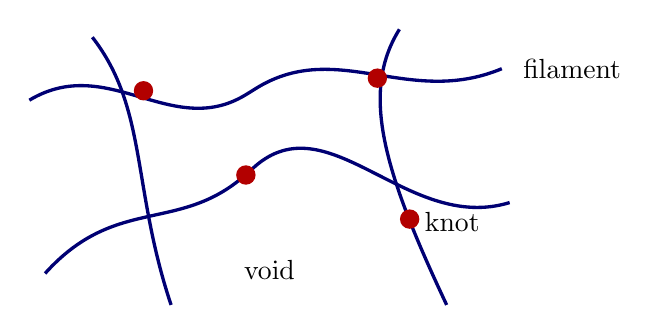
\begin{tikzpicture}[x=1cm,y=1cm]
  \draw[rounded corners=2pt,very thick,blue!45!black]
    (0.2,2.7) .. controls (1.2,3.3) and (2.0,2.2) .. (3.0,2.8)
    .. controls (4.1,3.5) and (5.0,2.6) .. (6.2,3.1);
  \draw[rounded corners=2pt,very thick,blue!45!black]
    (0.4,0.5) .. controls (1.3,1.5) and (2.1,1.0) .. (3.0,1.8)
    .. controls (4.0,2.7) and (5.0,1.0) .. (6.3,1.4);
  \draw[rounded corners=2pt,very thick,blue!45!black]
    (1.0,3.5) .. controls (1.7,2.6) and (1.5,1.6) .. (2.0,0.1);
  \draw[rounded corners=2pt,very thick,blue!45!black]
    (4.9,3.6) .. controls (4.4,2.8) and (4.7,1.8) .. (5.5,0.1);
  \fill[red!70!black] (1.65,2.82) circle (3.5pt);
  \fill[red!70!black] (4.62,2.98) circle (3.5pt);
  \fill[red!70!black] (2.95,1.75) circle (3.5pt);
  \fill[red!70!black] (5.03,1.19) circle (3.5pt);
  \node[align=center] at (3.25,0.55) {void};
  \node[right] at (6.35,3.1) {filament};
  \node[right] at (5.1,1.15) {knot};
\end{tikzpicture}\caption{카우스틱 그물망을 보여 주는 깔끔한 이차원 비유: 선 모양의 밀집 영역이 공동을 둘러싸고 더 밝은 매듭에서 만납니다. 삼차원에서는 기본 접힘이 시트를 이루고, 시트가 만나는 곳에 필라멘트와 마디가 생깁니다.}\label{fig:c09-caustic-network}\end{figure}

힘이 없는 이 구성은 우주론적 섭동 이론을 대체하지 않습니다. 밀도 대비의 성장, 헤일로와 은하의 형성, 비선형 구조에는 중력이 핵심적으로 작용합니다. 이 장난감 모형은 견고한 기하학적 사실 하나를 따로 드러냅니다. 초기 흐름이 조금만 달라도 자연스럽게 접히고 물질이 모인다는 사실입니다. 작은 초기 밀도 변화도 포함할 수 있으며, 그래도 야코비안에 관한 핵심 논증은 달라지지 않습니다.

그러므로 우리는 수수께끼를 없앤 것이 아니라 다른 곳으로 옮겼습니다. 급팽창은 어떤 영역을 늘려 매우 평탄하고 균일하게 만들기 위해 도입했습니다. 카우스틱 계산은 초기 흐름에 작은 속도 변화가 있다고 가정합니다. 이 비균질성의 씨앗은 어디서 왔을까요? 다음 강의에서는 급팽창 중 장의 양자 요동을 살펴보고, 그것이 어떻게 나중의 우주 그물 구조를 위한 초기 조건이 되는지 묻겠습니다.

\section{이 논증으로 확립한 내용}

균일한 스칼라 장은 퍼텐셜 \(V(\phi)\) 위를 움직이는 좌표처럼 거동합니다. 고정된 상자 안에서는 \(\ddot\phi=-V'(\phi)\)을 따릅니다. 팽창하는 공변 상자에서는 물리적 부피 \(a^3\)가 작용에 들어가 다음 식을 만듭니다.
\[
\ddot\phi+3H\dot\phi=-V'(\phi).
\]
허블 마찰은 장이 높고 완만한 퍼텐셜 위에서 느린 종단 운동을 하도록 붙들어 둘 수 있습니다. 그러면 장의 운동에너지는 무시할 수 있게 되고, 퍼텐셜 에너지는 \(H\)를 거의 일정하게 유지하며, \(a(t)\)는 대략 지수적으로 증가합니다.

팽창은 원치 않는 자기 홀극을 희석하고, 기하를 평탄하게 하며, 곡률을 영에 가깝게 만듭니다. 그러나 급팽창은 끝나야 합니다. 장은 고원을 벗어나 진동하고, 재가열 과정에서 뜨거운 입자에 에너지를 전달합니다. 퍼텐셜의 형태, 인플라톤의 정체와 초기 상태, 재가열 결합, 오늘날 관측되는 미소한 진공 에너지 등은 여전히 풀리지 않은 질문입니다.

급팽창의 성공은 마지막 질문을 낳습니다. 완벽하게 평탄해진 우주에는 은하가 하나도 없을 것입니다. 카우스틱 사상
\[
y=x+v(x)t,
\qquad
\frac{dn}{dy}=\frac{1}{1+v'(x)t}
\]
은 초기 흐름의 아주 작은 변화가 어떻게 날카로운 시트와 필라멘트, 매듭을 만들어 낼 수 있는지 보여 줍니다. 하지만 그러한 변화가 어디서 왔는지는 설명하지 않습니다. 이제 논의는 그 변화의 양자적 기원으로 넘어갑니다.
